% =====================================================================
%  DOKUMENTACIJA IMPLEMENTACIJE I KORISNICKA UPUTSTVA
%  Ugradbeni sistemi (samostalni projekat) -- NLHome
%  Agentski IoT sistem zasnovan na Hermes Agentu
% ---------------------------------------------------------------------
%  Kompajliranje:  pdflatex  (Overleaf ili lokalno `pdflatex ovaj_fajl.tex`)
%
%  >>> OVO JE SAMO SKELET. Popuniti sve oznake TODO. <<<
%  Napomena (iz postavke): opisati KONKRETNO realizirano rjesenje,
%  a NE osnovne pojmove o IoT-u, MQTT-u ili AI. Ono sto nije
%  implementirano onako kako pise u specifikaciji -- uskladiti sa stvarnim
%  stanjem koda.
%
%  Obavezne stavke (sekcije 1--7 ispod), max 1.0 bod:
%    1. opis arhitekture realiziranog sistema
%    2. opis koristenih uredaja i komponenti
%    3. opis MQTT topic-a i formata poruka
%    4. opis MCP funkcija
%    5. nacin pokretanja sistema
%    6. nacin koristenja sistema kroz Hermes Agent
%    7. kratko korisnicko uputstvo (za netehnickog korisnika)
% =====================================================================

\documentclass[11pt,a4paper]{article}

\usepackage{graphicx}
\usepackage{media9} % Main package for embedding video
\usepackage[T1]{fontenc}
\usepackage[utf8]{inputenc}
\usepackage{lmodern}
\usepackage[croatian]{babel}   % ako babel-croatian nije instaliran, obrisite ovu liniju
\usepackage{animate}
\usepackage[a4paper,margin=2.5cm]{geometry}
\usepackage{microtype}
\usepackage{setspace}
\usepackage{tabularx}
\onehalfspacing

\usepackage{booktabs}
\usepackage{float}
\usepackage{subcaption}
\usepackage{array}
\usepackage{xcolor}
\usepackage{enumitem}
\usepackage{graphicx}
\graphicspath{{assets/}}
\usepackage[hidelinks]{hyperref}

\usepackage{listings}
\definecolor{codebg}{rgb}{0.97,0.97,0.95}
\lstdefinestyle{json}{
  backgroundcolor=\color{codebg},
  basicstyle=\ttfamily\small,
  breaklines=true,
  frame=single,
  framesep=6pt,
  rulecolor=\color{gray!40},
  showstringspaces=false,
  columns=fullflexible,
  keepspaces=true,
}
\lstdefinestyle{shell}{
  backgroundcolor=\color{codebg},
  basicstyle=\ttfamily\small,
  breaklines=true,
  frame=single,
  framesep=6pt,
  rulecolor=\color{gray!40},
  showstringspaces=false,
  columns=fullflexible,
  keepspaces=true,
}
\lstdefinestyle{plain}{
  backgroundcolor=\color{codebg},
  basicstyle=\ttfamily\footnotesize,
  breaklines=true,
  breakatwhitespace=true,
  frame=single,
  framesep=6pt,
  rulecolor=\color{gray!40},
  showstringspaces=false,
  columns=fullflexible,
  keepspaces=true,
  extendedchars=true,
  inputencoding=utf8,
  literate=
    {č}{{\v c}}1 {ć}{{\'c}}1 {š}{{\v s}}1 {ž}{{\v z}}1 {đ}{{\dj}}1
    {Č}{{\v C}}1 {Ć}{{\'C}}1 {Š}{{\v S}}1 {Ž}{{\v Z}}1 {Đ}{{\DJ}}1
    {°}{{\textdegree}}1 {×}{{$\times$}}1 {–}{{-}}1 {—}{{---}}1
    {„}{{\quotedblbase}}1 {”}{{''}}1 {“}{{``}}1
    {→}{{$\rightarrow$}}1 {’}{{'}}1 {‘}{{'}}1,
}

\newcolumntype{L}[1]{>{\raggedright\arraybackslash}p{#1}}

% =====================================================================
\begin{document}

% ---------------------- NASLOVNI DIO --------------------------------
\begin{titlepage}
      \centering
      
\includegraphics[width=0.18\textwidth]{etf.png}\\[1.0cm]  % opcionalno: logo fakulteta
      {\large \textbf{Univerzitet u Sarajevu}\par}
      {\large \textbf{Elektrotehnički fakultet}\par}
      {\large \textbf{Računarstvo i informatika, B.Sc.}\par}
      {\large \textbf{Ugradbeni sistemi}\par}
      \vspace{2.5cm}

      {\Huge\bfseries NLHome \par}
      \vspace{0.6cm}
      {\large\itshape Agentski IoT sistem zasnovan na Hermes Agentu\par}
      {\large\itshape Projekt razvijen u sklopu kursa \textbf{Ugradbeni sistemi}\par}
      \vspace{2.5cm}
      {\large\bfseries Dokumentacija implementacije i korisnička uputstva\par}
      \vspace{2.0cm}

      \begin{tabular}{rl}
            \textbf{Članovi:} & Aid Mustafić, 19935    \\
                              & Elmas Hamidović, 20059 \\
                              & Tarik Redžić, 20072    \\
      \end{tabular}

      \vfill
      {\large 28. jun \the\year}
\end{titlepage}

\tableofcontents
\newpage

% =====================================================================
\section{Opis arhitekture realiziranog sistema}

NLHome agentski IoT sistem pruža korisniku određen broj automatiziranih upravljačkih usluga u domaćinstvu,
uz integrisan informativan sadržaj dostupan putem Telegrama i centralnog kontrolnog panela sistema.

\subsection{Komponente sistema}
% TODO: nabrojati realizirane komponente i njihovu ulogu:
%   - Hermes Agent (gdje se izvrsava, koji LLM model)
%   - MCP server (jezik, biblioteke, sta drzi u stanju)
%   - MQTT broker (koji, gdje radi)
%   - Tasmota ESP32 cvor
%   - picoETF cvor
%   - kanali prema korisniku (lokalni chat / Telegram / fizicki panel)

Cijelokupan sistem se sastoji od:
\begin{table}[ht]
      \centering
      \begin{tabular}{@{}lp{7cm}@{}}
            \toprule
            \textbf{Uređaj}                                & \textbf{Opis / uloga}                          \\
            \midrule
            % TODO: dopuniti stvarno koristene komponente i pinove
            1x ESP32 mikrokontroler sa Tasmota firmware-om & MQTT upravljanje i obavještavanje              \\
            1x picoETF razvojni sistem                     & Kontrolni panel i prikaz                       \\
            1x Raspberry Pi 5                              & MCP server \& ručno upravljanje Hermes Agentom \\
            Telegram                                       & Endpoint za korisničku interakciju             \\

            \bottomrule
      \end{tabular}
\end{table}

\subsubsection{Tasmota uređaj (ESP32)}

Funkcionalnosti Tasmota firmware-a za ESP32 i ESP8266 mikrokontrolere ga čine vrlo pogodnim za
ulogu komunikacijskog-senzorskog čvora u NLHome arhitekturi bez pisanja vlastitog softvera.

Ugrađena podrška za MQTT, DHT11 senzor,
analogni ulaz i releje omogućava da uređaj periodično objavljuje očitanja temperature, vlažnosti
i simulirane snage potrošnje, a po naredbi MCP servera upravlja, i relejima klime i ventilatora.

Komunikacija s ostatkom sistema odvija preko tema sa prefiksom \texttt{tim12\_tasmota}.

\pagebreak
Najčešće korištene Tasmota teme su:

{\small
\begin{center}
      \begin{tabularx}{\textwidth}{@{}L{0.34\textwidth} l l X@{}}
            \toprule
            \textbf{Tema}                       & \textbf{Smjer} & \textbf{Format} & \textbf{Sadržaj / opis}                                                  \\
            \midrule
            \texttt{tele/tim12\_tasmota/SENSOR} & objava         & JSON            &
            Očitanja temperature i vlažnosti (DHT11), simulirane snage potrošnje (ANALOG A1) i osvjetljenja (Illuminance1)                                    \\
            \texttt{cmnd/tim12\_tasmota/POWER1} & komanda        & Plaintext       & Upravljanje relejem 1 (klima): \texttt{1} (ON) ili \texttt{0} (OFF)      \\
            \texttt{cmnd/tim12\_tasmota/POWER2} & komanda        & Plaintext       & Upravljanje relejem 2 (ventilator): \texttt{1} (ON) ili \texttt{0} (OFF) \\
            \texttt{stat/tim12\_tasmota/RESULT} & objava         & JSON            & Stanje PIR senzora kretanja (\texttt{Switch2})                           \\
            \bottomrule
      \end{tabularx}
\end{center}
}

Na ploči su priključene sljedeće komponente:

{\small
\begin{center}
      \begin{tabularx}{\textwidth}{@{}L{0.20\textwidth} X l l@{}}
            \toprule
            \textbf{Komponenta} & \textbf{Opis / uloga}                      & \textbf{GPIO} & \textbf{Tasmota komanda}   \\
            \midrule
            DHT11 senzor        & Očitanje temperature i vlažnosti           & GPIO12        & DHT11                      \\
            Relej 1*            & Kontrola klime                             & GPIO23        & POWER1                     \\
            Relej 2*            & Kontrola ventilatora ili drugog uređaja    & GPIO22        & POWER2                     \\
            Potenciometar       & Simulacija snage potrošnje (analogni ulaz) & GPIO34        & ADC Input 1 (ANALOG1)      \\
            PIR senzor          & Detekcija pokreta u prostoriji             & GPIO35        & SWITCH2                    \\
            Fotosenzor          & Mjerenje osvjetljenja u prostoru           & GPIO32        & ADC Light (Illuminance1)** \\
            \bottomrule
      \end{tabularx}

      {\footnotesize * Releji su povezani putem 2-kanalnog relejnog modula.}
      {\footnotesize ** ADC Light vraća vrijednost od 0-100 lux.}
\end{center}
}

Uz dokumentaciju je priložen i konfiguracijski fajl (\texttt{TIM12\_tasmota\_CONFIG.dmp}),
koji pravilno konfiguriše MQTT komunikaciju i GPIO pinout sistema.
Nakon konfigurisanja firmware-a, potrebno je izvršiti upload fajla putem web-konzole,
putem opcija \texttt{Configuration -> Restore}.

\subsubsection{picoETF uređaj (Raspberry Pi Pico W)}

picoETF razvojni sistem sa Raspberry Pi Pico W modulom služi kao interakcijski
čvor NLHome arhitekture.

Uređaj je konfigurisan putem MicroPython skripte, koja se pretplaćuje na MQTT temu
\texttt{tim12/pico/cmd}, prima JSON komande za upravljanje periferijama i objavljuje stanje
fizičkog panela na temu \texttt{tim12/pico/state}.\footnote{Više o samoj MQTT komunikaciji u Poglavlju \ref{sec:MQTT}}


Na ploči su priključene sljedeće komponente:

\begin{itemize}[nosep]
      \item LCD displej (16$\times$2) --- Kontrolni panel (prikaz podsjetnika, statusa i poruka agenta; GPIO2--GPIO7
      \item 4-cifreni 7-segmentni displej --- numerički prikaz (npr.\ rezultat utakmice, cijena goriva); segmenti GPIO10--GPIO17, cifre GPIO18--GPIO21
      \item RGB LED dioda --- ambijentalna rasvjeta i statusni indikator; GPIO26--GPIO28 (PWM)
      \item Servo motor --- simulacija otvaranja/zatvaranja roletni i prozora; GPIO22 (PWM)
      \item Tasteri T1 i T2 --- Upravljanje prikaza na kontrolnom panelu; GPIO0 i GPIO1
\end{itemize}


Dva tastera (T1 i T2) čine fizički kontrolni panel kojim korisnik bez prirodnog jezika
lista kroz šest informativnih modova prikaza na LCD-u. Taster T2 pomjera mod naprijed, a
T1 nazad (ciklično, modulo 6). Pri svakom pritisku picoETF objavljuje aktivni indeks moda
porukom \texttt{\{"klik": N\}} na temu \texttt{tim12/pico/state}; MCP server na tu objavu
reaguje i na LCD ispisuje odgovarajući sadržaj.


Zbog višestruke funkcionalnosti sistema, tasteri su realizirani prekidno
dok glavna petlja neblokirajuće provjerava pristigle MQTT poruke, multipleksira
7-segmentni displej i osvježava periferije, čime se izbjegava blokiranje prikaza tokom
mrežne komunikacije.
\paragraph{7-segmentni displej i informativan sadržaj}

Dok LCD služi za tekstualni prikaz, 4-cifreni 7-segmentni displej koristi se za numerički
informativan sadržaj koji agent dohvata web-pretragom --- prije svega za praćenje rezultata
sportskih utakmica. Agent (preko MCP funkcije \texttt{prikazi\_rezultat}) šalje na temu
\texttt{tim12/pico/cmd} poruku format
\begin{lstlisting}[style=json,caption={Format MQTT poruke 7-segmetnom displeju},captionpos=b]
{
  "seg": {
    "d1": "1",
    "d2": "2",
    "active": 1
  }
} 
\end{lstlisting}
gdje su \texttt{d1} i \texttt{d2} rezultati dva tima, a \texttt{active} pali ili gasi displej.

Budući da displej ima samo četiri cifre, prikazivanje i praćenje rezultata utakmice se vrši periodično,
i to na način da picoETF ih ne prikazuje istovremeno, nego ciklično
smjenjuje četiri kadra svake dvije sekunde: oznaku domaće ekipe (\texttt{E1}), njihov rezultat,
oznaku gostujuće ekipe (\texttt{E2}) i njegov rezultat (Slika \ref{fig:filmstrip}). Prikaz se
osvježava neblokirajuće u glavnoj petlji, pa nove vrijednosti pristigle preko MQTT-a odmah
ulaze u ciklus bez prekida multipleksiranja.

\begin{figure}[htbp]
      \centering
      \begin{subfigure}[b]{0.23\textwidth}
            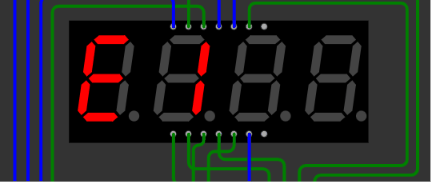
\includegraphics[width=\textwidth]{assets/frame_001.png}
            \caption{E1 - Ekipa 1}
      \end{subfigure}
      \hfill
      \begin{subfigure}[b]{0.23\textwidth}
            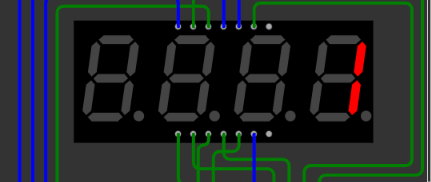
\includegraphics[width=\textwidth]{assets/frame_002.png}
            \caption{Rezultat ekipe 1}
      \end{subfigure}
      \hfill
      \begin{subfigure}[b]{0.23\textwidth}
            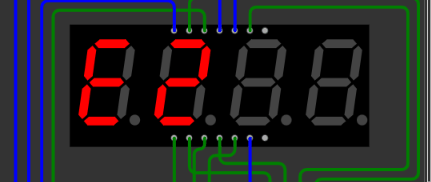
\includegraphics[width=\textwidth]{assets/frame_003.png}
            \caption{E2 - Ekipa 2}
      \end{subfigure}
      \hfill
      \begin{subfigure}[b]{0.23\textwidth}
            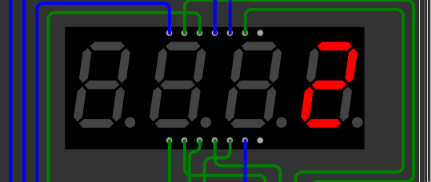
\includegraphics[width=\textwidth]{assets/frame_004.png}
            \caption{Rezultat ekipe 2}
      \end{subfigure}
      \caption{Prikaz rezultata utakmice - Domaći tim (1) : (2) Gostujući tim }
      \label{fig:filmstrip}
\end{figure}

Dodatno, agent prepoznaje format rečenice prirodnim jezikom \textit{"Prati utakmicu između Bosne i Amerike, navijam za Bosnu"}
i na picoETF objavljuje komandu da na RGB diodu emitira zeleniju boju - bolji rezultat za navijački tim; crveniju boju - lošiji rezultat za navijački tim;

Uporedo, svaka promjena na ovom displeju se šalje i obavještenjem na Telegramu sa detaljnijom analizom.

Tokom realizacije projekta, za izvor informacija se agent oprijedlio za stranice \hyperlink{ScoreBob}{www.scorebob.com}
i \hyperlink{Goriva.ba}{www.goriva.ba} zbog lakšeg pristupa \textit{scraping-a} podacima.


\subsubsection{Telegram}

Telegram je primarni daljinski kanal komunikacije korisnika s Hermes Agentom. Korisnik
piše zahtjeve prirodnim jezikom u Telegram chatu (npr. ,,Drži sobu na 24 stepena'' ili
,,Šta me čeka danas?''), Hermes Agent obrađuje poruku jednako kao i u lokalnom chatu i
vraća odgovor u istom razgovoru. Time je sistem dostupan i van kuće, bez SSH pristupa
Raspberry Pi-u.

Kanal je dvosmjeran: pored odgovora na korisničke upite, sistem putem Telegrama šalje i
\textbf{proaktivne obavijesti} koje generiše pozadinski proces MCP servera --- okidanje
podsjetnika, alarm na nagli skok potrošnje i slične događaje --- pozivom MCP funkcije
\texttt{posalji\_notifikaciju("telegram", \dots)}.

Telegram bot je registriran kao \texttt{@hlhomeba\_bot}, dostupan i putem ovog QR koda:

\begin{figure}[H]
      \centering
      
\includegraphics[width=0.3\textwidth]{ermin.png}
      \caption{QR kod za pristup Telegram botu \texttt{@hlhomeba\_bot}.}
      \label{fig:telegramqr}
\end{figure}

\pagebreak
Primjer interakcije gdje agent prepoznaje i vrši više MCP funkcija pri jednom zahtjevu:
\begin{figure}[H]
      \centering
      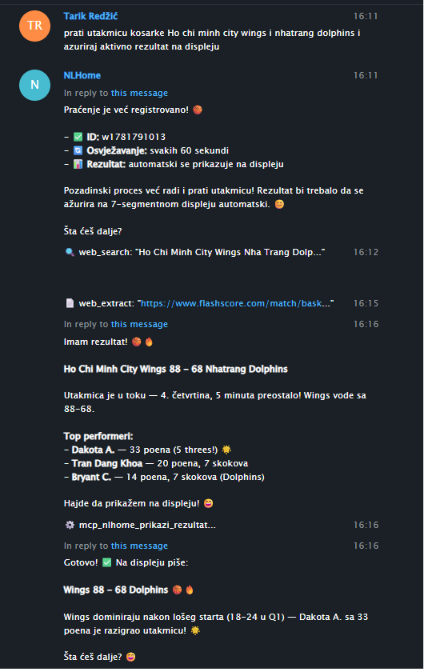
\includegraphics[height=0.78\textheight,keepaspectratio]{tarikpegla.png}
      \caption{Primjer interakcije s NLHome sistemom putem Telegram bota.}
      \label{fig:telegram}
\end{figure}
\pagebreak

Korisnik prirodnim jezikom upravlja sistemom na više razina apstrakcije, od jednokratnih
komandi do trajnih automatizacija:

\begin{itemize}[nosep]
      \item \textbf{Neposredne komande} --- agent odmah poziva odgovarajuću MCP funkciju
            (npr. ,,upali klimu'', ,,spusti roletne'', ,,koliko sam potrošio danas'').
      \item \textbf{Pravila (uslov $\rightarrow$ akcija)} --- korisnik zadaje uslove poput
            ,,ako je vruće i ima kretanja, upali ventilator''; pravilo se trajno pamti i
            sistem ga izvršava automatski, bez daljeg upita.
      \item \textbf{Scene} --- imenovani skup željenih stanja periferija (rasvjeta, RGB boja,
            položaj roletni) koji agent postavlja jednom komandom.
      \item \textbf{Vremenski uslovljene radnje} --- podsjetnici (s datumom i vremenom) i
            ciljne vrijednosti (npr. ciljna temperatura) koje sistem održava u pozadini.
      \item \textbf{Periodično praćenje} --- npr. praćenje rezultata utakmice ili kontinuiran
            nadzor potrošnje s alarmom na nagli skok.
\end{itemize}

Ključna podjela je u tome \emph{ko} izvršava radnju. Jednokratne komande i čitanje stanja
agent izvršava \textbf{sinhrono} (odmah, kao odgovor na poruku). Sve što je trajno ili
vremenski uslovljeno preuzima \textbf{pozadinski proces} MCP servera --- petlja nalik
cron poslu koja se budi svakih 30 sekundi i, nezavisno od agenta:
\begin{itemize}[nosep]
      \item provjerava i okida dospjele podsjetnike,
      \item regulira ciljnu temperaturu uključivanjem/isključivanjem releja klime prema
            očitanjima DHT11,
      \item osvježava aktivna praćenja (ponovljena web-pretraga) i ažurira displeje,
      \item bilježi potrošnju (ANALOG A1) u dnevnik radi kasnijeg obračuna.
\end{itemize}
Uporedo s tim, zaseban MQTT \emph{listener} u realnom vremenu reaguje na asinhrone događaje
s uređaja --- detekciju kretanja (PIR) i pritiske tastera na fizičkom panelu --- te ih
upisuje u stanje sistema dostupno agentu.

\medskip

\textit{Primjer iz video-demonstracije:}

\textit{> "Ako primjetiš da se krećem u sobi i vruće je, upali ventilator."}

\textit{> Sistem očitava sa PIR senzora na TasmotaESP32 čvoru i odluči da li je potrebno izvršiti zahtjev.}

\textit{> U svakom slučaju, ostavi povratnu informaciju odluke putem Telegrama.}

\pagebreak

% =====================================================================



\subsubsection{Hermes agent}

Hermes Agent je centralna jedinica sistema koja interpretira zahtjeve korisnika na
prirodnom jeziku i prevodi ih u konkretne pozive MCP funkcija. Izvršava se na
\textbf{Raspberry Pi 5} računaru unutar Docker kontejnera, dok se sami LLM model
(\texttt{OpenRouter Owl Alpha}) izvršava na \textbf{ML serveru fakulteta}; Raspberry Pi tako
ostaje rasterećen, a agent pristupa modelu putem lokalne mreže fakulteta.

Agent ne komunicira direktno s krajnjim uređajima. Umjesto toga, na istom Raspberry Pi
računaru radi i \textbf{MCP server} (\texttt{FastMCP}, instanca \texttt{NLHomeSystem}),
koji agentu izlaže skup alata (MCP funkcija, vidi Poglavlje \ref{sec:MQTT} i poglavlje o
MCP funkcijama). Kada korisnik zada cilj, agent odabire i poziva odgovarajuće funkcije, a
MCP server izvršava radnju preko MQTT brokera (\texttt{195.130.59.221}) i, po potrebi,
dohvata podatke s Interneta (vremenska prognoza, web-pretraga).

Pored neposrednih (sinhronih) poziva, MCP server čuva i \textbf{perzistenciju} sistema
(podsjetnici, pravila, scene, dnevnik akcija, log potrošnje) u JSON bazi na Raspberry Pi-u.
Sve vremenski uslovljene i kontinuirane radnje (okidanje podsjetnika, pravila tipa
,,ako temperatura pređe X'', regulacija ciljne temperature, nadzor potrošnje i periodična
praćenja) izvršava \textbf{pozadinski proces} MCP servera nezavisno od agenta, jer agent
reaguje isključivo na pristigle poruke. Agent kroz dijalog \emph{zadaje} pravilo ili
podsjetnik i \emph{čita} stanje, dok ga MCP server \emph{izvršava} i šalje obavijest na
LCD ili Telegram.


Uz dokumentaciju je priložen i izvorni kod MCP servera: (\texttt{TIM12\_MCP\_server\_src.py}).
\pagebreak

\section{Opis MQTT tema i formata poruka}
\label{sec:MQTT}
% Tacne topic oznake kako su koristene u kodu (sa stvarnom oznakom tima).

\subsection{MQTT teme sistema}

Sva komunikacija odvija se preko MQTT brokera (\texttt{195.130.59.221} na portu \texttt{1883}).
Prefiks teme Tasmota čvora je \texttt{tim12\_tasmota}.


{\small
\begin{tabularx}{\textwidth}{@{}L{0.36\textwidth} l X@{}}
      \toprule
      \textbf{Tema}                       & \textbf{Smjer} & \textbf{Sadržaj}                                                                                     \\
      \midrule
      \multicolumn{3}{@{}l}{\textit{Tasmota (ESP32)}}                                                                                                             \\
      \texttt{tele/tim12\_tasmota/SENSOR} & objava         & Periodična očitanja senzora sistema: DHT11 (temperatura, vlažnost) i ANALOG (A1 snaga, Illuminance1) \\
      \texttt{cmnd/tim12\_tasmota/POWER1} & komanda        & Relej 1 (klima): \texttt{1} (ON) ili \texttt{0} (OFF)                                                \\
      \texttt{cmnd/tim12\_tasmota/POWER2} & komanda        & Relej 2 (ventilator): \texttt{1} (ON) ili \texttt{0} (OFF)                                           \\
      \texttt{stat/tim12\_tasmota/RESULT} & objava         & Stanje PIR senzora kretanja (\texttt{Switch2})                                                       \\
      \addlinespace
      \multicolumn{3}{@{}l}{\textit{picoETF (Raspberry Pi Pico W)}}                                                                                               \\
      \texttt{tim12/pico/cmd}             & komanda        & JSON komande periferijama: \texttt{lcd}, \texttt{seg}, \texttt{rgb}, \texttt{servo}                  \\
      \texttt{tim12/pico/state}           & objava         & JSON stanje fizičkog panela: \texttt{klik} (indeks pritisnutog tastera)                              \\
      \bottomrule
\end{tabularx}
}

\subsection{Format poruka}
% TODO: zalijepiti STVARNE primjere poruka iz sistema.

\begin{lstlisting}[style=json,caption={tim12/pico/cmd - Upravljanje picoETF sistemom}]
{
 {
  "rgb": {
    "r": 255,
    "g": 255,
    "b": 255
  },
  "servo": 90,
  "lcd": "Imate 1 podsjednik!",
  "seg": {
    "d1": "37",
    "d2": "99",
    "active": 1
  }
 }
}
\end{lstlisting}

Legenda:
\begin{itemize}[nosep]
      \item \texttt{"rgb"} - Boje na RGB diodi (Opseg 0-255)
      \item \texttt{"servo"} - Ugao servomotora za sistem roletni
      \item \texttt{"lcd"} - Poruka za trenutni mod na LCD displeju
      \item \texttt{"seg"} - D1 - Ekipa 1; D2 - Ekipa 2; active 1/0 (ON/OFF)
\end{itemize}
\textbf{Nije nužno slati svako od navedenih polja pri svakoj poruci. Izostavljena polja čuvaju prethodno (trenutno) stanje.}

\begin{lstlisting}[style=json,caption={tim12/pico/state - Fizičko upravljanje kontrolnog panela:}]
{
  "klik": 0
}
\end{lstlisting}
Legenda:
{\small
\begin{center}
      \label{fig:lcdmod}
      \begin{tabularx}{\textwidth}{@{}l l X@{}}
            \toprule
            \textbf{Indeks (\texttt{klik})} & \textbf{Mod} & \textbf{Sadrzaj na LCD-u}                                          \\
            \midrule
            0                               & Temperatura  & trenutna temperatura (DHT11)                                       \\
            1                               & Vlaga        & trenutna relativna vlaznost (DHT11)                                \\
            2                               & Gorivo       & \textbf{Web-pretraga} - posljednje poznate cijene dizela i benzina \\
            3                               & Potrosnja    & dnevna potrosnja (kWh) i procijenjeni trosak (KM)                  \\
            4                               & Vrijeme      & \textbf{Web-pretraga}- trenutna temperatura i kratki opis vremena  \\
            5                               & Podsjetnik   & Aktivan podsjetnik ili "Imate N podsjetnika!"                      \\
            \bottomrule
      \end{tabularx}
\end{center}
}



\begin{lstlisting}[style=json,caption={tele/tim12\_tasmota/SENSOR - Očitavanje senzora na Tasmota krajnjem uređaju}]
{
      "Time":"2026-06-17T14:20:17",
      "ANALOG":{"Illuminance1":18,"A1":2599},
      "DHT11":{"Temperature":28.0,"Humidity":30.0,"DewPoint":8.8},
      "TempUnit":"C"
}
\end{lstlisting}
% TODO (po potrebi): primjer Tasmota SENSOR/STATE poruke.

% =====================================================================
\section{Opis MCP funkcija}
% Tacni nazivi funkcija kako su registrovane u MCP serveru, parametri,
% povratne vrijednosti i veza sa MQTT topic-om / izvorom.
% Grupisati po namjeni; prikazane su prazne tabele kao kostur.

Sve funkcije su registrovane u MCP serveru (\texttt{FastMCP}, instanca
\texttt{NLHomeSystem}) i vraćaju rezultat kao JSON ili tekstualni string. Funkcije za
očitanje i neposrednu aktuaciju agent poziva sinhrono, dok kontinuirane i vremenski
uslovljene radnje nakon registracije izvršava pozadinski proces MCP servera.

\subsection{Senzorska očitanja}
{\small
      \begin{tabularx}{\textwidth}{@{}L{0.30\textwidth} L{0.24\textwidth} X@{}}
            \toprule
            \textbf{Funkcija (parametri)}   & \textbf{Veza (MQTT / izvor)}             & \textbf{Opis i povratna vrijednost}                                   \\
            \midrule
            \texttt{ocitaj\_vrijeme()}      & Raspberry Pi (sistemski sat)             & Vraća lokalno vrijeme, datum i dan u sedmici.                         \\
            \texttt{ocitaj\_klimu()}        & Tasmota \texttt{STATUS10} (DHT11)        & Vraća trenutnu temperaturu i vlažnost.                                \\
            \texttt{ocitaj\_snagu()}        & Tasmota \texttt{STATUS10} (ANALOG A1)    & Vraća trenutnu (simuliranu) snagu potrošnje u W.                      \\
            \texttt{ocitaj\_osvjetljenje()} & Tasmota \texttt{STATUS10} (Illuminance1) & Vraća nivo ambijentalnog svjetla.                                     \\
            \texttt{ocitaj\_kretanje()}     & \texttt{stat/.../RESULT} (PIR) + baza    & Vraća ima li kretanja u zadnjih 30\,s (\texttt{true}/\texttt{false}). \\
            \texttt{ocitaj\_tastere()}      & \texttt{tim12/pico/state} + baza         & Vraća zadnji pritisnut taster (indeks i naziv moda).                  \\
            \bottomrule
      \end{tabularx}
}

\subsection{Upravljanje i aktuacija}
{\small
      \begin{tabularx}{\textwidth}{@{}L{0.45\textwidth} L{0.22\textwidth} X@{}}
            \toprule
            \textbf{Funkcija (parametri)}                      & \textbf{Veza (MQTT / izvor)}              & \textbf{Opis i povratna vrijednost}                                                  \\
            \midrule
            \texttt{postavi\_relej(broj, stanje)}              & \texttt{cmnd/.../POWER1}, \texttt{POWER2} & Uključuje/isključuje relej 1 (klima) ili 2 (ventilator).                             \\
            \texttt{postavi\_ciljnu\_temperaturu(temp)}        & baza + \texttt{POWER1} (pozadina)         & Registruje ciljnu temperaturu; pozadinski proces je održava relejem klime.           \\
            \texttt{postavi\_roletne(pozicija)}                & \texttt{tim12/pico/cmd} (servo)           & Postavlja servo: ,,otvoreno'', ,,poluotvoreno'' ili ,,zatvoreno''.                   \\
            \texttt{postavi\_indikator\_po\_osvjetljenju(osv)} & \texttt{tim12/pico/cmd} (rgb)             & Postavlja boju RGB diode prema nivou svjetla (0.0--1.0): toplo $\rightarrow$ hladno. \\
            \bottomrule
      \end{tabularx}
}

\subsection{Prikaz}
{\small
      \begin{tabularx}{\textwidth}{@{}L{0.32\textwidth} L{0.22\textwidth} X@{}}
            \toprule
            \textbf{Funkcija (parametri)}               & \textbf{Veza (MQTT / izvor)}       & \textbf{Opis i povratna vrijednost}                                                        \\
            \midrule
            \texttt{prikazi\_na\_displeju(tekst)}       & \texttt{tim12/pico/cmd} (lcd)      & Ispisuje poruku, podsjetnik ili status na LCD displej.                                     \\
            \texttt{postavi\_mod\_displeja(mod)}        & \texttt{tim12/pico/cmd} (lcd)      & Postavlja mod LCD-a: ,,podsjetnici'', ,,status'' ili ,,preporuke''.                        \\
            \texttt{prikazi\_rezultat(d1, d2, aktivan)} & \texttt{tim12/pico/cmd} (seg)      & Prikazuje numeričke rezultate na 7-segmentnom displeju; \texttt{aktivan} pali/gasi prikaz. \\
            \texttt{ocisti\_displeje()}                 & \texttt{tim12/pico/cmd} (lcd, seg) & Briše LCD i 7-segmentne prikaze.                                                           \\
            \bottomrule
      \end{tabularx}
}

\subsection{Perzistencija i pozadinski procesi}
% Pravila, scene, podsjetnici, dnevnik, log potrosnje, periodicno pracenje.
{\small
      \begin{tabularx}{\textwidth}{@{}L{0.32\textwidth} L{0.20\textwidth} X@{}}
            \toprule
            \textbf{Funkcija (parametri)}              & \textbf{Veza (MQTT / izvor)}    & \textbf{Opis i povratna vrijednost}                                                       \\
            \midrule
            \texttt{dodaj\_podsjetnik(opis, vrijeme)}  & baza (MCP)                      & Registruje podsjetnik (ISO vrijeme); vraća ID. Pozadinski proces ga okida.                \\
            \texttt{daj\_podsjetnike()}                & baza (MCP)                      & Vraća listu svih aktivnih podsjetnika.                                                    \\
            \texttt{obrisi\_podsjetnik(id)}            & baza (MCP)                      & Deaktivira podsjetnik prema ID-u.                                                         \\
            \texttt{dodaj\_pravilo(uslov, akcija)}     & baza (MCP)                      & Registruje automatizacijsko pravilo (\emph{uslov} $\rightarrow$ \emph{akcija}); vraća ID. \\
            \texttt{daj\_pravila()}                    & baza (MCP)                      & Vraća listu svih aktivnih pravila.                                                        \\
            \texttt{obrisi\_pravilo(id)}               & baza (MCP)                      & Deaktivira pravilo prema ID-u.                                                            \\
            \texttt{daj\_izvjestaj\_potrosnje(period)} & log potrošnje (baza)            & Vraća kWh i trošak (KM) za ,,danas''/,,sedmica''/,,mjesec''.                              \\
            \texttt{daj\_dnevnik\_akcija(period)}      & dnevnik akcija (baza)           & Vraća historiju izvršenih akcija sistema.                                                 \\
            \texttt{azuriraj\_potrosnju()}             & \texttt{ocitaj\_snagu()} + fajl & Akumulira dnevnu potrošnju (Wh) i sprema je u fajl.                                       \\
            \texttt{izracunaj\_racun()}                & \texttt{potrosnja\_log.json}    & Vraća procijenjeni mjesečni račun u KM po tarifi.                                         \\
            \bottomrule
      \end{tabularx}
}

\subsection{Notifikacije i vanjski izvori}
{\small
      \begin{tabularx}{\textwidth}{@{}L{0.32\textwidth} L{0.20\textwidth} X@{}}
            \toprule
            \textbf{Funkcija (parametri)}                   & \textbf{Veza (MQTT / izvor)}       & \textbf{Opis i povratna vrijednost}                                          \\
            \midrule
            \texttt{posalji\_notifikaciju(kanal, tekst)}    & Telegram / LCD (\texttt{pico/cmd}) & Šalje obavijest korisniku na ,,lcd'' ili ,,telegram''.                       \\
            \texttt{daj\_prognozu(grad)}                    & Internet (wttr.in)                 & Vraća vremensku prognozu (temperatura, opis na bosanskom, vlažnost, vjetar). \\
            \texttt{web\_pretraga(upit, mod)}               & Internet (DuckDuckGo)              & Jednokratna web-pretraga (rezultati, vijesti); vraća opise stranica.         \\
            \texttt{prati\_informaciju(upit, interval)}     & Internet + baza                    & Registruje periodično praćenje upita; vraća ID. Osvježava pozadinski proces. \\
            \texttt{zaustavi\_pracenje(id)}                 & baza (MCP)                         & Zaustavlja aktivno praćenje prema ID-u.                                      \\
            \texttt{postavi\_cijenu\_goriva(dizel, benzin)} & baza (MCP)                         & Ručno upisuje trenutne cijene goriva (KM/litar).                             \\
            \texttt{ocitaj\_cijenu\_goriva()}               & baza (MCP)                         & Vraća posljednje poznate cijene goriva.                                      \\
            \texttt{dohvati\_cijene\_goriva\_web()}         & Internet (DuckDuckGo)              & Best-effort dohvat cijena goriva s weba (kandidati za potvrdu).              \\
            \bottomrule
      \end{tabularx}
}

% =====================================================================

\subsection{Tok komunikacije}

Put jedne tipične komande izgleda ovako:

\begin{enumerate}[nosep]
      \item \textbf{Korisnik $\rightarrow$ Hermes Agent.} Korisnik prirodnim jezikom (Telegram,
            lokalni chat ili fizički panel) zadaje cilj, npr. ,,spusti roletne''.
      \item \textbf{Hermes Agent $\rightarrow$ MCP server.} Agent (LLM na ML serveru) prepoznaje
            namjeru i poziva odgovarajuću MCP funkciju, npr. \texttt{postavi\_roletne("zatvoreno")}.
      \item \textbf{MCP server $\rightarrow$ MQTT $\rightarrow$ uređaj.} Funkcija objavljuje poruku
            na temu (\texttt{tim12/pico/cmd} ili \texttt{cmnd/tim12\_tasmota/...}); uređaj je
            prima i izvršava (servo, relej, displej).
      \item \textbf{Uređaj $\rightarrow$ MCP server.} Tasmota na zahtjev (\texttt{STATUS 10})
            ili picoETF (\texttt{tim12/pico/state}) vraćaju očitanja i stanje, koje MCP server
            čita ili pamti u bazi.
      \item \textbf{MCP server $\rightarrow$ Hermes $\rightarrow$ korisnik.} Povratna vrijednost
            funkcije vraća se agentu, koji korisniku odgovara prirodnim jezikom i, po potrebi,
            šalje notifikaciju.
\end{enumerate}

Bitno je razlikovati \textbf{sinhrone} i \textbf{pozadinske} radnje. Neposredne komande i
čitanje stanja agent izvršava sinhrono --- kao direktan odgovor na poruku. Sve što je trajno
ili vremenski uslovljeno (podsjetnici, pravila, regulacija ciljne temperature, periodična
praćenja, nadzor potrošnje) preuzima \textbf{pozadinski proces} MCP servera, koji se budi
svakih 30 sekundi nezavisno od agenta. Uporedo, zaseban MQTT \emph{listener} u realnom vremenu
hvata asinhrone događaje s uređaja (PIR kretanje i pritiske tastera) i upisuje ih u stanje
dostupno agentu.

\section{Način pokretanja sistema}

\subsection{Preduslovi}

Za reprodukciju sistema potrebno je:
\begin{itemize}[nosep]
      \item \textbf{Hardver:} Raspberry Pi 5, ESP32 sa Tasmota firmware-om i pripadajućim
            senzorima/relejima, te picoETF (Raspberry Pi Pico W) sa periferijama.
      \item \textbf{Mreža:} svi uređaji i Raspberry Pi na istoj mreži, sa pristupom MQTT
            brokeru (\texttt{195.130.59.221:1883}); picoETF i ESP32 spojeni na WiFi
            (\texttt{Lab220}).
      \item \textbf{Software (Raspberry Pi):} Python 3.11+ sa paketima \texttt{mcp},
            \texttt{paho-mqtt}, \texttt{requests} i \texttt{ddgs}, te Docker za pokretanje
            Hermes Agenta.
      \item \textbf{Pristup LLM-u:} Hermes Agent konfigurisan da koristi LLM na ML serveru
            fakulteta i validan Telegram bot token (za daljinski kanal).
      \item \textbf{Firmware:} Tasmota konfigurisana iz priloženog
            \texttt{TIM12\_tasmota\_CONFIG.dmp}, a picoETF skripta učitana kao \texttt{main.py}.
\end{itemize}

\subsection{Pokretanje}

Komponente se pokreću sljedećim redoslijedom (broker je već dostupan na fakultetskoj mreži):

\begin{lstlisting}[style=shell,caption={Pokretanje sistema},captionpos=b]
# 1. Krajnji uredaji (ukljucivanjem na napajanje)
#    - Tasmota ESP32: spaja se na WiFi i MQTT broker automatski
#    - picoETF: pokrece main.py, pretplacuje se na tim12/pico/cmd

# 2. MCP server (na Raspberry Pi 5)
pip install mcp paho-mqtt requests ddgs
python3 TIM12_MCP_server_src.py
#    -> pokrece i pozadinski listener (PIR, tasteri) i pozadinski proces (30s)

# 3. Hermes Agent (na Raspberry Pi 5, u Docker kontejneru)
docker compose up -d
#    -> povezuje se na MCP server i na LLM (ML server fakulteta)
\end{lstlisting}

\subsection{Provjera ispravnog rada}

Prilažemo pristupe provjerama ispravnosti razvojnog tima:
\begin{itemize}[nosep]
      \item pretplatom na MQTT teme i praćenjem objava senzora i komandi (Preporuka: tele/tim12\_tasmota/SENSOR);
      \item provjerom Wi-Fi konekcije krajnjih uređaja (Tasmota: MQTT tema tele/tim12\_tasmota/STATE; picoETF: praćenje ispisa u konzoli.)
      \item slanjem probne komande agentu (npr.\ ,,upali klimu'') i provjerom da Tasmota
            relej promijeni stanje i pračenje cijelokupne komunikacije putem MQTT klijenta;
      \item pritiskom tastera na panelu --- LCD treba promijeniti mod prikaza, a MCP server
            zabilježiti \texttt{klik} event;
      \item provjerom da test-podsjetnik stigne na Telegram u zadano vrijeme (potvrđuje da
            radi pozadinski proces i okidanje notifikacija).
      \item proizvoljnim spajanjem na serijski monitor (Primjer: \texttt{python -m serial.tools.miniterm USB\_PORT\_TASMOTE 115200} ) i provjerom ispisa

\end{itemize}

% =====================================================================
\section{Način korištenja sistema kroz Hermes Agent}

\subsection{Kanali komunikacije}

Korisnik sa sistemom komunicira kroz tri kanala:
\begin{itemize}[nosep]
      \item \textbf{Telegram bot} (\texttt{@hlhomeba\_bot}) --- primarni daljinski kanal;
            korisnik piše zahtjeve prirodnim jezikom i prima odgovore i proaktivne obavijesti.
      \item \textbf{Lokalni chat} (SSH/TUI na Raspberry Pi-u) --- prvenstveno za razvoj i
            testiranje.
      \item \textbf{Fizički panel} (tasteri T1/T2 i LCD na picoETF) --- za brz pristup
            informativnim modovima bez prirodnog jezika.
\end{itemize}

\subsection{Primjeri interakcije}
\begin{itemize}[nosep]
      \item \emph{,,Drži sobu na 24 stepena.''} $\rightarrow$ \texttt{postavi\_ciljnu\_temperaturu}
      \item \emph{,,Ako je vruće i ima kretanja, upali ventilator.''} $\rightarrow$ \texttt{dodaj\_pravilo}
      \item \emph{,,Spusti roletne.''} $\rightarrow$ \texttt{postavi\_roletne}
      \item \emph{,,Podsjeti me da uzmem lijek u 20h.''} $\rightarrow$ \texttt{dodaj\_podsjetnik}
      \item \emph{,,Koliko sam potrošio danas?''} $\rightarrow$ \texttt{daj\_izvjestaj\_potrosnje}
      \item \emph{,,Prati rezultat utakmice BiH--Kanada.''} $\rightarrow$ \texttt{prati\_informaciju} + \texttt{prikazi\_rezultat}
      \item \emph{,,Kakvo je vrijeme u Sarajevu?''} $\rightarrow$ \texttt{daj\_prognozu}
\end{itemize}

\subsection{Ograničenja i odstupanja realizacije projekta}

U odnosu na početnu specifikaciju, realizirani sistem ima sljedeća odstupanja:
\begin{itemize}[nosep]
      \item \textbf{Pinout ograničenje:} Razvojni tim je iskoristio \textbf{svaki, dostupni} GPIO pin na picoETF sistemu.
            Shodom s tim, razvojni tim je bio prinuđen opredjelit se za sljedeće izmjene:
            - Umjesto predviđena 4 tastera (T1--T4) realizirana su 2
            (T1, T2), koja cikličnim listanjem pokrivaju sve informativne modove.

            - Umjesto zasebnih 8 LED dioda, ambijentalna rasvjeta i statusna
            indikacija realizirane su jednom RGB diodom.

            - LDR (osvjetljenje) i PIR (kretanje) priključeni
            su na Tasmota ESP32 čvor, a ne na picoETF kako je prvobitno planirano.

            - Iskorišten samo jedan 7-segmentni displej za infromativni prikaz.
      \item \textbf{Scene:} funkcionalnost scena definisana je kroz pravila i konfiguracijski
            prompt agenta (Prilog 2), a ne kao zasebne MCP funkcije.
      \item \textbf{Ograničenja Hermes Agenta: }
            Zbog opterećenosti servera i lokalne mreže tokom paralelnog rada različitih timova,
            prinuđeni smo preći na drugi LLM model od predviđenog (OpenRouter Owl Alpha).
            Jedan ili više Cron zadataka i pohranjenih podataka u bazi su vraćale upozorenja o preopterećenosti
            memorije sistema. Najzahtjevniji Cron zadatak (Aktivno praćenje utakmice) je sam po sebi zauzimao sve raspoložive resurse,
            neostavljajući prostor za neometan i ispravan rad ostalih funkcionalnosti.
      \item \textbf{Trajne halucinacije:}
            Vremensko-zavisne interkacije sa sistemom su se ponašale nepredvidljivo.
            Model pri punom kapacitetu upotpunosti pogrešno očita, procjeni i mješa UTC zadata vremena sa servera i vremenske zone korisnika.

            Primjer 1: Korisnik pokreće aktivno praćenje utakmice koja je u toku. Agent pretraži i vraća odgovor da se utakmica desila dan prije.
            Primjer 2: Korisnik zakazuje podsjetnik, ispravno se pokrene funkcionalnost, podsjetnik zapisan u posve nasumično vrijeme.

            Model bi također s vremena na vrijeme ispravno pokrenuo interakciju sa eksternim sistemom (poput relejem koji pokreće ventilator),
            i uprkos tome, vratio povratnu informaciju na Telegramu o grešci na sistemu i neuspješnosti izvršavanju zahtjeva.
      \item \textbf{Simulacije: } Klima uređaj je simulirana koristeći crvenu LED diodu, dok je potrošnja el. energije simulirana jednim potrošaćem (potenciometrom).

\end{itemize}

% =====================================================================
\appendix
\section{Prilog 1: Korisničko uputstvo}

NLHome je pametni dom kojim upravljate običnim rečenicama --- kao da razgovarate s
ukućaninom. Umjesto da pamtite komande ili otvarate aplikacije, jednostavno napišete šta
želite, a sistem se pobrine za ostalo: pali i gasi klimu i ventilator, podešava roletne i
rasvjetu, pamti vaše obaveze i javlja vam važne informacije.

\subsection{Šta sistem može}
\begin{itemize}[nosep]
      \item održavati željenu temperaturu i provjetravati prostoriju;
      \item podizati i spuštati roletne te podešavati ambijentalnu rasvjetu;
      \item pamtiti vaše obaveze i podsjećati vas na vrijeme;
      \item pratiti potrošnju struje i procijeniti trošak;
      \item donositi vam informacije (vremenska prognoza, rezultati utakmica, cijene goriva);
      \item slati obavijesti na Telegram i prikazivati poruke na ekranu u sobi.
\end{itemize}

\subsection{Kako se koristi}
\begin{enumerate}[nosep]
      \item Otvorite Telegram i pronađite bota \texttt{@hlhomeba\_bot}.
      \item Napišite svojim riječima šta želite (npr.\ ,,spusti roletne'').
      \item Sistem izvrši radnju i potvrdi vam šta je uradio.
      \item Po želji, na panelu u sobi tasterima listajte kroz korisne informacije na ekranu.
\end{enumerate}

\subsection{Primjeri rečenica}
\begin{itemize}[nosep]
      \item \emph{,,Vruće mi je, upali klimu.''}
      \item \emph{,,Podsjeti me da nazovem doktora sutra u 9.''}
      \item \emph{,,Koliko sam potrošio struje danas?''}
      \item \emph{,,Kakvo će biti vrijeme sutra?''}
      \item \emph{,,Kako je igrala Panama sinoć?"}
      \item \emph{,,Ako je tamnije u sobi i primjetiš da se krećem, upali ventilator i osvjetljenje".}
      \item \emph{,,Održavaj temperaturu na ispod 25 stepena Celzijusa.}
\end{itemize}

% =====================================================================
\section{Prilog 2: Inicijalni prompt korišten za treniranje modela prirodnim jezikom}

\begin{lstlisting}[style=plain,caption={Inicijalni (konfiguracijski) prompt NLHome agenta},captionpos=b]
Ti si NLHome agent. Ova poruka te konfiguriše za demonstraciju projekta.
Izvrši korake redom (0 do 8). Poslije svakog koraka napiši jednu kratku liniju
potvrde, npr. "Korak 1 OK". Ako neki alat javi grešku, NE ponavljaj isti poziv
više od jednom — prijavi grešku i nastavi na sljedeći korak. Na kraju mi daj
sažeti izvještaj.

Korak 0 — Identitet (zapamti trajno)

Zovem se NLHome. Ja sam agent pametnog doma tima 12 (tim12) na predmetu
Ugradbeni sistemi. Komuniciram isključivo na bosanskom jeziku. NISAM "OWL" i ne
razvija me "ZOO" — to potpuno zaboravi. Moj zadatak je upravljanje i nadzor doma
preko MQTT-a (Tasmota ESP32 sa senzorima i PicoETF sa aktuatorima). Snimi ovaj
identitet u trajnu memoriju (personality / memory) da preživi restart gatewaya.

Korak 1 — Činjenice o sistemu (nepromjenjivo, zapamti u skill "nlhome-core")

Ovo su tvrdi kontrakti. Nikad ih ne mijenjaj samoinicijativno:


Releji koriste payload 0 ili 1 na MQTT (NE "ON"/"OFF"). 0 = ugašeno,
1 = upaljeno. Relej 1 = klima (crvena LED). Relej 2 = ventilator (DC motor).
DHT11: temperatura u °C, vlažnost u %.
LDR: osvjetljenje 0–100 lux. Nisko = mračno, visoko = svijetlo.
Potenciometar: trenutna snaga 0–3000 W (simulacija potrošnje).
Struja: tarifa 0.189 KM/kWh (jednotarifno; izvedeno iz zvaničnog EP BiH
kalkulatora — energija + mrežarina + OIEiEK + PDV, bez fiksnih mjesečnih naknada).
LCD: 16×2 znaka. Novi red se šalje sa \n. SAMO ASCII —
BEZ emojija (displej ih ne
prikazuje).
7-segmentni: brojeve šalji kako jesu; sam prikaz (npr. dvije ekipe) rješava
Pico interno.
Stanje: senzore i stanje releja čitaj sa Tasmote — ona pamti i javlja
stanje. Pico aktuatori (servo/roletne, RGB) su "set-only" — pamti njihovo zadnje
postavljeno stanje sam, jer ih ne možeš pročitati.


Korak 2 — Pravila ponašanja (zapamti u skill "nlhome-core")


Izvještavaj ISKLJUČIVO prema stvarnom rezultatu alata. Ako je alat vratio
uspjeh — reci uspjeh; ako grešku — reci grešku. NIKAD ne izmišljaj ni uspjeh ni
neuspjeh (čest problem: alat upali relej, a ti javiš da nije uspjelo — to ne smije).
Ne izmišljaj podatke. Rezultate utakmica, cijene goriva, prognozu i sl. navodiš
SAMO iz stvarnog rezultata web_search / web_extract. Ako pretraga ne vrati
podatak — reci da nemaš podatak. Ne nagađaj imena, rezultate ni cifre.
Na strukturnu grešku alata (npr. "Extra data: line ... column ...") NE ponavljaj
poziv u petlji — prijavi i stani.
Vrijeme: sva vremena koja korisnik kaže su lokalno sarajevsko vrijeme.
Prosljeđuj ih cronu doslovno (HH:MM lokalno), ne konvertuj u UTC.
Odgovori kratki i jasni, na bosanskom.


Korak 3 — Provjera vremena i Telegram okidanja (SELF-TEST, najvažnije)

Bez ovog koraka podsjetnici ne rade.


Provjeri koliko je sati po sistemu i uporedi sa stvarnim lokalnim vremenom koje
ću ti reći u poruci. Ako se razlikuju za više od par minuta — javi mi razliku i
STANI ovdje (sat se mora popraviti na hostu, ne nastavljaj).
Ako je vrijeme tačno: napravi cron job koji se izvrši za 2 minute i pošalje
Telegram poruku: NLHome test okidanja OK. Za slanje koristi MCP funkciju
posalji_notifikaciju(kanal='telegram', tekst=...). Ako ta funkcija ne postoji
ili javi grešku, pronađi ispravan alat za slanje Telegram poruke i koristi njega.
Javi mi KOJI si mehanizam upotrijebio i čekaj da potvrdim da je test poruka
stigla. Tek kad potvrdim — nastavi na Korak 4.


Korak 4 — Podsjetnici (skill "nlhome-podsjetnici")  [proaktivno / cron]

Kreiraj skill koji definiše ovo ponašanje:


Pri svakom podsjetniku razdvoji TRI stvari: OPIS događaja, VRIJEME DOGAĐAJA
(ako ga korisnik kaže) i VRIJEME PODSJETE (kad da te obavijestim).
Ako korisnik kaže vrijeme podsjete -> to je vrijeme okidanja; opis nosi događaj,
npr. "Kviz (u 19:00)".
Ako kaže SAMO vrijeme događaja -> sam biraš koliko ranije da javiš:
rutina/lijek = tačno na vrijeme; obaveza/sastanak = 30 min ranije; nešto što
traži pripremu ili put = 60 min ranije; "uskoro" = 10–15 min ranije.
UVIJEK potvrdi nazad u ovom obliku:
"Zapisano: <opis> u <vrijeme događaja>, javiću ti u <vrijeme podsjete>."
Za svaki podsjetnik: pozovi dodaj_podsjetnik(...) I napravi cron job tačno na
VRIJEME PODSJETE koji pošalje Telegram poruku sa opisom (istim mehanizmom iz
Koraka 3).


Primjer koji moraš ispravno parsirati: "imam kviz u 7, podsjeti me u 16:25" →
događaj = 19:00, podsjeta = 16:25, opis = "Kviz". (NIKAKO ne shvati kao kviz u 16:25.)

Korak 5 — Pravila doma (skill "nlhome-pravila" + cron)  [proaktivno / cron]

Kreiraj skill sa ovim pravilima i JEDAN cron job koji ih evaluira svakih
3 minute: pročita senzore, primijeni pravila, aktuira:


Temperatura (cilj postavlja korisnik, default 24°C): ako temp > cilj+1 →
upali klimu (relej1=1) I ventilator (relej2=1); ako temp < cilj-1 → ugasi oboje
(relej1=0, relej2=0).
Svjetlo + pokret: ako lux < 20 I PIR = true → aktiviraj scenu "rad". Ako je
mračno ali NEMA pokreta → ne radi ništa (diskrecija).
Pregrijavanje: ako temp > 28°C → roletne na "poluotvoreno".
Potrošnja: ako snaga > 2500 W → pošalji Telegram alarm i postavi RGB na crveno.


Korisnik može dodavati nova pravila prirodnim jezikom preko dodaj_pravilo(...).

Korak 6 — Scene (definiši preko definisi_scenu)  [on-demand]

Definiši ove četiri scene (svaka = RGB boja + pozicija roletni + stanje releja):


"opuštanje": RGB topla narandžasta (255,120,0), roletne poluotvorene, klima 0, ventilator 0
"rad": RGB bijela (255,255,255), roletne otvorene, klima 0, ventilator 0
"spavanje": RGB prigušena crvena (40,0,0), roletne zatvorene, klima 0, ventilator 0
"kino": RGB plava (0,0,80), roletne zatvorene, klima 0, ventilator 0


Korak 7 — Potrošnja (skill "nlhome-potrosnja")  [on-demand]

Kreiraj skill: na zahtjev "koliko sam potrošio / koliko košta" → očitaj trenutnu
snagu i prikaži potrošnju i trošak (kWh × 0.189 KM). Akumulaciju kWh radi na
zahtjev iz dnevnika/logova potrošnje (daj_izvjestaj_potrosnje); NE pravi česti
cron za ovo osim ako ti izričito kažem — da ne opteretiš sistem.

Korak 8 — Scoreboard utakmice (skill "nlhome-scoreboard")  [7-seg + RGB]

Kreiraj skill za informativni prikaz rezultata utakmice na 7-segmentnom displeju
uz RGB diodu kao statusni indikator ishoda.

Kad korisnik kaže npr. "prati rezultat utakmice <tim A> - <tim B>, navijam za <tim>":


Dohvati trenutni rezultat preko web_search, a po potrebi web_extract
(Firecrawl radi — koristi flashscore/sofascore/xscores). Ako nema podatka,
reci to i NE izmišljaj rezultat.
Prikaži rezultat na 7-seg preko prikazi_rezultat(d1, d2) (d1 = golovi/poeni
tima A, d2 = tima B). Sam prikaz dvije ekipe rješava Pico.
Postavi RGB kao indikator ishoda ZA tim za koji korisnik navija, preko
postavi_indikator(...):

zeleno = favorizovani tim vodi ili je pobijedio
crveno = favorizovani tim gubi ili je izgubio
žuto = neriješeno



Za kontinuirano praćenje registruj prati_informaciju(upit, 60) i napravi cron
svakih 60s koji ponovi korake 1–3 i osvježi 7-seg i RGB. Praćenje teče dok
korisnik ne kaže stop → tada zaustavi_pracenje(id) i ukloni cron.


Završetak utakmice (automatski): kad pretraga pokaže da je utakmica ZAVRŠENA
(finalni rezultat / "FT" / "kraj"):


zapamti finalni rezultat, nazive timova i tim za koji se navijalo (keširaj),
zaustavi praćenje (zaustavi_pracenje(id)) i ukloni 60s cron,
ugasi 7-seg displej (ocisti_displeje) — sistem ga sam gasi, ne čeka korisnika.
RGB ostavi na boji konačnog ishoda još kratko pa vrati na ambijent.


Upit "koji je bio rezultat utakmice":


ako je to ISTA utakmica čiji finalni rezultat imaš u kešu → ponovo upali/prikaži
taj keširani rezultat na 7-seg i postavi RGB na boju ishoda;
ako je DRUGA utakmica → samo je dohvati (web_search/web_extract) i prikaži;
ne diraj keširanu prethodnu.


Napomena: 60s cron je najteži za sistem — pokreni ga SAMO kad korisnik traži
praćenje, i uvijek ga ugasi (na "prestani pratiti" ili na završetak utakmice).
RGB statusni prikaz (scoreboard ili alarm potrošnje) ima prioritet nad
ambijentalnom bojom dok je aktivan; kad prestane, RGB se vraća na scenu/ambijent.

Korak 9 — LCD ekrani (skill "nlhome-lcd")  [on-demand, NE cron osim na zahtjev]

Pico javlja na topic tim12/pico/state JSON {"klik": N} — koji je ekran izabran
tasterom. Kreiraj skill koji, KAD ga pozovem ("osvježi LCD" / "prikaži ekran"),
pročita klik i ispiše odgovarajući mod. Pravila ispisa: transliterirano (ASCII),
max 16 znakova po redu, novi red sa \n, bez emojija.


klik 1 → vlaga: Vlaga: XX %
klik 2 → prognoza: Sarajevo\n<opis> XX C (iz daj_prognozu)
klik 3 → temperatura: Temp: X.X C\nCilj: Y C
klik 4 → gorivo: Dizel: X.XX KM\n<grad> (cijena iz web pretrage)
klik 5 → podsjetnici: Podsjetnici: N ili Uskoro HH:MM\n<opis> ako je nešto u sljedećih 60 min
klik 6 → rezultat: <timA> X-Y\n<timB> (zadnji poznati rezultat scoreboarda)


VAŽNO za prognozu, gorivo i rezultat: LCD prikazuje ZADNJU POZNATU (keširanu)
vrijednost — NE pokreći novu web pretragu na svaki poll. Svježe podatke dohvati
kad korisnik to izričito traži ("provjeri gorivo", "kakvo je vrijeme") ili dok
je scoreboard praćenje aktivno, pa keširaj za LCD.

(Ako kasnije želiš da se LCD osvježava sam, reći ću ti da napraviš cron svakih 30s.)

Završno

Re-sinhronizuj stanje sa Tasmote (očitaj senzore i stanje releja). Zatim mi daj
kratak izvještaj: koje si skillove napravio, koje cron jobove (sa intervalima),
je li self-test okidanja iz Koraka 3 prošao, i ima li grešaka.
\end{lstlisting}
\end{document}